\section{Results}
\label{sec:results}

All numbers are generated from \texttt{results/v2/summary.json}; intervals are 95\% hierarchical
bootstrap CIs. Analyses added after pre-registration are marked exploratory. Example episodes and predictions are in
\Cref{fig:world} (Appendix~\ref{app:extra}).


\begin{figure*}[t]
\centering
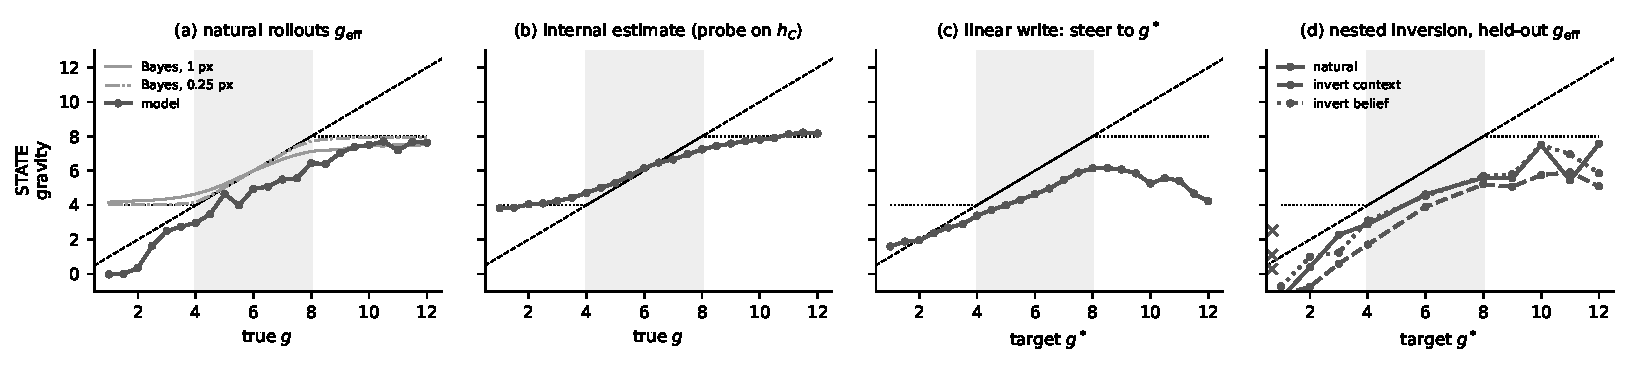
\includegraphics[width=0.72\textwidth]{fig_locus.pdf}
\caption{Where the out-of-range failure lives. Rows: families. (a) Natural predictions, with the
Bayes-optimal reference (grey). (b) The gravity a linear probe reads from the belief. (c) Linear
write: predictions after steering the belief so that the probe reads $g^\star$. (d) Nested inversion
on held-out frames: natural, inverted context latents and inverted belief; the crosses at the left
are the anti-physics control ($g=-4$). Dashed: the law; dotted: the clamp.}
\label{fig:locus}
\end{figure*}

\subsection{Competence gate and decodability (E0, E1)}
\label{sec:competence}

\Cref{tab:competence} reports the pre-registered competence gate (in-range slope of
$g_{\rm eff}$ against $g$ on validation episodes) and probe decodability. STATE \StateGate{} the
gate (slope \StateSlope), REC \RecGate{} (\RecSlope) and JEPA \JepaGate{} (\JepaSlope).
Gravity is linearly decodable from the trained belief at $R^2$ \StateRtwoG{} (STATE), \RecRtwoG{}
(REC) and \JepaRtwoG{} (JEPA), against \StateRtwoGun{}, \RecRtwoGun{} and \JepaRtwoGun{} for an
untrained dynamics network on the same inputs. H1 demanded $R^2\ge 0.5$ and is supported only for
STATE (Holm $p$: \PHOneState, \PHOneRec, \PHOneJepa). Energy at the last context frame is
decodable at $R^2$ \StateRtwoE{}, \RecRtwoE{} and \JepaRtwoE{} (Appendix~\ref{app:extra}), as
Proposition~\ref{prop:decode} predicts for any competent predictor.

\begin{table}[t]
\centering\small
\caption{Competence and decodability (M size, $10^5$ episodes, mean over seeds).}
\label{tab:competence}
\setlength{\tabcolsep}{3pt}
\begin{tabular}{lcccccc}
\toprule
Family & seeds & slope & err$_8$ (px) & $R^2_g$ & $R^2_g$ untr. & $R^2_E$\\
\midrule
STATE & \StateSeeds & \StateSlope & \StateErrEight & \StateRtwoG & \StateRtwoGun & \StateRtwoE\\
REC   & \RecSeeds   & \RecSlope   & \RecErrEight   & \RecRtwoG   & \RecRtwoGun   & \RecRtwoE\\
JEPA  & \JepaSeeds  & \JepaSlope  & \JepaErrEight  & \JepaRtwoG  & \JepaRtwoGun  & \JepaRtwoE\\
\bottomrule
\end{tabular}
\end{table}


\subsection{Natural out-of-range response (E2)}
\label{sec:natural}

\Cref{fig:locus}(a) shows the gravity that natural predictions exhibit as the true gravity sweeps
from 1 to 12, together with the Bayes-optimal reference of Proposition~\ref{prop:clamp}. The
pre-registered normalized slopes ($1$ = law, $0$ = clamp) are
$\rho_{\rm hi}=$ \StateNatHi{} for STATE, \RecNatHi{} for REC and \JepaNatHi{} for JEPA.
H2 predicted $\rho<0.5$ on both sides and is \emph{not supported} for any family (\Cref{tab:hyp}, Appendix~\ref{app:extra}).
On the high side the STATE estimate is below 0.5 but its interval crosses it, and the pixel-family
intervals are too wide to say anything. On the low side the estimates exceed one
(\StateNatLo, \RecNatLo, \JepaNatLo). This is an artifact: at low gravity the models predict floor contacts that the slow reference
never makes, and the curvature fit reads them as extra acceleration (Appendix~\ref{app:details}).

The exploratory law fraction $\lambda$ (Appendix~\ref{app:lambda}; projection of the prediction onto the law-minus-clamp
counterfactual difference; all frames, no curvature fit) gives a tighter and plainer picture
(\Cref{tab:lambda}). On the high side natural predictions sit roughly half-way between clamp and
law: \StateLambdaNatHi{} (STATE), \RecLambdaNatHi{} (REC), \JepaLambdaNatHi{} (JEPA). On the low
side they sit near the clamp: \StateLambdaNatLo{}, \RecLambdaNatLo{}, \JepaLambdaNatLo. The models
neither clamp as the noisy-Bayes reference does nor follow the law, and they extrapolate upward
better than downward.


\begin{table}[t]
\centering\small
\caption{Exploratory law fraction $\lambda$ (1 = law, 0 = clamp). ``nat'' and ``write'' use all 20
predicted frames; the last four columns use only the held-out frames 4--13 of the inversion
episodes. WIDE is the same architecture trained on $g\sim\mathcal U[1,12]$ (one seed): an
empirical ceiling.}
\label{tab:lambda}
\setlength{\tabcolsep}{3.5pt}
\begin{tabular}{llcccccc}
\toprule
 & & \multicolumn{2}{c}{all frames} & \multicolumn{4}{c}{held-out frames}\\
\cmidrule(lr){3-4}\cmidrule(lr){5-8}
side & family & nat & write & nat & inv-$z$ & inv-$h$ & WIDE\\
\midrule
high & STATE & \StateLamNatHiPt & \StateLamSteerHiPt & \StateHoldNatHi & \StateHoldInvZHi & \StateHoldInvHHi & \StateHoldWideHi\\
     & REC   & \RecLamNatHiPt & \RecLamSteerHiPt & \RecHoldNatHi & \RecHoldInvZHi & \RecHoldInvHHi & \RecHoldWideHi\\
     & JEPA  & \JepaLamNatHiPt & \JepaLamSteerHiPt & \JepaHoldNatHi & \JepaHoldInvZHi & \JepaHoldInvHHi & \JepaHoldWideHi\\
\midrule
low  & STATE & \StateLamNatLoPt & \StateLamSteerLoPt & \StateHoldNatLo & \StateHoldInvZLo & \StateHoldInvHLo & \StateHoldWideLo\\
     & REC   & \RecLamNatLoPt & \RecLamSteerLoPt & \RecHoldNatLo & \RecHoldInvZLo & \RecHoldInvHLo & \RecHoldWideLo\\
     & JEPA  & \JepaLamNatLoPt & \JepaLamSteerLoPt & \JepaHoldNatLo & \JepaHoldInvZLo & \JepaHoldInvHLo & \JepaHoldWideLo\\
\bottomrule
\end{tabular}
\end{table}

\subsection{Locating the failure (E3)}
\label{sec:locus}

\paragraph{Internal estimate.} The probe's reading of out-of-range gravity
(\Cref{fig:locus}b) has normalized slope
(\Cref{fig:locus}b) is the best-measured quantity in the study. Its normalized slope is
\StateInfHi{} (STATE), \RecInfHi{} (REC) and \JepaInfHi{} (JEPA) on the high side, and
\StateInfLo{}, \RecInfLo{}, \JepaInfLo{} on the low side. The belief tracks out-of-range gravity
but under-reads it: by about half above the range and by about a third below it. On the high side
this matches what the predictions do ($\lambda\approx 0.5$--$0.7$), so there the belief holds no
more than the output shows. On the low side the belief reads far more gravity change than the
predictions express ($\lambda\le 0.3$): information is present and unused. One caveat: a linear
probe fit in range under-reads by a similar factor on frozen V-JEPA~2 features of the same frames
(\VjRhoHi{} on the high side; Appendix~\ref{app:extra}), so part of the under-reading may be the
geometry of the code and not a clamped belief.

\paragraph{Linear write.} Steering along the matched-pair direction transfers in range with slope
$s_{\rm exe}=$ \StateExeS{} (STATE), \RecExeS{} (REC), \JepaExeS{} (JEPA), and reduces the error
to the simulator's counterfactual by CER $=$ \StateCer{}, \RecCer{}, \JepaCer{}. H3 (validity of
the write) is supported only for STATE (Holm $p$: \PHThreeState, \PHThreeRec, \PHThreeJepa), so we
interpret steering only there. For STATE, writing the true gravity raises the high-side law fraction
from \StateLamNatHiPt{} to \StateLamSteerHiPt, the level of the WIDE model trained on that range
(\StateWideLamHi). On the low side it moves only from \StateLamNatLoPt{} to \StateLamSteerLoPt{}
(WIDE: \StateWideLamLo).

\paragraph{Nested inversion.} The pre-registered inversion slopes do not resolve anything. With the
belief optimized (inv-$h$), held-out $\rho_{\rm hi}$ is \StateInvHHi{} (STATE), \RecInvHHi{} (REC)
and \JepaInvHHi{} (JEPA), and the other cells are as wide. The pre-registered decision
rule returns \StateLocusHi/\RecLocusHi/\JepaLocusHi{} above the range and
\StateLocusLo/\RecLocusLo/\JepaLocusLo{} below it (STATE/REC/JEPA). We report the labels because we committed to them and do not lean on them: across the 21
configurations of Appendix~\ref{app:extra} they change with no pattern.

In the law fraction on the same held-out frames (\Cref{tab:lambda}, right) the picture is
asymmetric. On the low side, optimizing the belief helps every family (STATE
\StateHoldNatLo{}$\to$\StateHoldInvHLo, REC \RecHoldNatLo{}$\to$\RecHoldInvHLo, JEPA
\JepaHoldNatLo{}$\to$\JepaHoldInvHLo): beliefs exist that make the frozen decoder continue a
low-gravity trajectory better than the natural belief does, and for STATE the frozen belief network
does not reach them from any context latents we could find (inv-$z$ \StateHoldInvZLo). On the high
side inversion gains little for STATE (\StateHoldNatHi{}$\to$\StateHoldInvHHi) and loses for the
pixel families. The anti-physics control reaches $\lambda=$ \StateAntiLam, \RecAntiLam{} and
\JepaAntiLam{} of the way to an upward-gravity trajectory on held-out frames. The decoder can be
bent a third of the way toward dynamics it has never seen, which bounds how much of any inversion
gain can be credited to stored physics.

\paragraph{An empirical ceiling (exploratory).} The WIDE model shows what this architecture does
when the same gravities are in range. Its in-range error equals the main model's (STATE
\StateInErrWide{} vs \StateInErr{} px; REC \RecInErrWide{} vs \RecInErr), so the wider prior costs
nothing. Out of range the main models lose \StateOodErrHi{} vs \StateOodErrWideHi{} px (STATE, high)
and \StateOodErrLo{} vs \StateOodErrWideLo{} px (low). Even WIDE reaches only $\lambda=$ \StateHoldWideHi{} on
held-out frames, so a quarter of the ``law'' is beyond this architecture at any range. Of the gap
between the natural model and WIDE, the optimized belief closes \StateGapHHi{} (high) and
\StateGapHLo{} (low) for STATE, \RecGapHLo{} (low) for REC and \JepaGapHLo{} (low) for JEPA.

\paragraph{Reading.} No single locus survives. The evidence splits the failure in two. Part is
\emph{inference}: the belief under-reads out-of-range gravity, tightly measured, in every family.
Part is \emph{execution}: even the best belief we can find closes about half of the gap to a
model trained on the range, or less. The one validated write (STATE, high side) recovers the ceiling, which suggests that this
family's high-side failure is mostly inference; inversion cannot confirm it, because a
four-frame fit barely constrains gravity. On the low side execution is the larger part.

\paragraph{Perception is not the locus.} Positions read from context latents of out-of-range
episodes exceed the in-range readout error by \RecPercExcess{} px (REC) and \JepaPercExcess{} px
(JEPA) (H5 supported).

\subsection{Scale and controls (E7)}
\label{sec:scaling}

\Cref{fig:scaling} (Appendix~\ref{app:extra}) varies the training pool from $10^3$ to $10^5$ episodes. In-range error falls by
about two pixels per decade in every family (\StateHfourErr; \RecHfourErr; \JepaHfourErr).
The slope of $\rho_{\rm hi}$ per decade is \StateHfourRho{} (STATE), \RecHfourRho{} (REC) and
\JepaHfourRho{} (JEPA). H4 required the upper bound to stay below 0.15 and is \emph{not supported}.:
we cannot claim that scale fails to buy extrapolation. The exploratory law fraction points the
other way for data. High-side $\lambda$ rises with the pool for STATE (\StateOneKLamHi,
\StateEightKLamHi{} and \StateLamNatHiPt{} at $10^3$, $8{\cdot}10^3$ and $10^5$ episodes), and the
low side leaves the clamp (\StateOneKLamLo{} to \StateLamNatLoPt). More data
bought some extrapolation here. Dynamics size did not, and a linear diagonal recurrence in place of the GRU lowered it
(STATE \StateLruLamHi; one seed each).


\subsection{Pre-registered tests}

Of seventeen confirmatory tests, four survive Holm correction (\Cref{tab:hyp}, Appendix~\ref{app:extra}): decodability and
steering validity for STATE, and the perception check for both pixel families. Secondary results (energy drift, velocity edits,
other shifts) are in Appendix~\ref{app:extra}: no family conserves energy, and we found no linear handle on
horizontal velocity.
